\documentclass{article}
\usepackage[utf8]{inputenc}
%\usepackage{biblatex}
\usepackage{amssymb}
\usepackage{amsmath}
\usepackage{amsthm}
\usepackage{graphicx}
\usepackage{float}
\usepackage{url}
\usepackage{framed}
\usepackage{booktabs}
\usepackage{enumitem}
\usepackage{extarrows}
%\usepackage{algorithm}
%\usepackage{algorithmic}
\usepackage[ruled,linesnumbered]{algorithm2e}
\numberwithin{equation}{section}
%\usepackage{BOONDOX-calo}
\title{ Partially coherent ptychography}
%\author{huibinchang }
\date{July 2021}

\begin{document}

\maketitle
\tableofcontents

\section{Models}



\subsection{Coherent model}
\begin{equation}
\label{basic}
f_{j}=\left|\mathcal{F}\left( \mathcal{S}_{j} u  \circ \omega \right)\right|^{2} 
\end{equation}

In a discrete setting, $u \in \mathbb{C}^{n}$ is a 2D image with $\sqrt{n} \times \sqrt{n}$ pixels, $\omega \in \mathbb{C}^{\bar{m}}$ is a localized 2D probe with $\sqrt{\bar{m}} \times \sqrt{\bar{m}}$ pixels.

$f_{j} \in \mathbb{R}_{+}^{\bar{m}}(\forall 0 \leq j \leq J-1)$ is a stack of phaseless measurements. Here $|\cdot|$ represents the element-wise absolute value of a vector, o denotes the elementwise multiplication, and $\mathcal{F}$ denotes the normalized 2 dimensional discrete Fourier transform. Each $\mathcal{S}_{j} \in \mathbb{R}^{\bar{m} \times n}$ is a binary matrix that crops a region $j$ of size $\bar{m}$ from the image $u$.

In practice, as the probe is almost never completely known, one has to solve a blind ptychographic phase retrieval (BP-PR) problem:

 To find $\omega \in \mathbb{C}^{\bar{m}}$ and $u \in \mathbb{C}^{n}$ s.t. $|\mathcal{A}(\omega, u)|=\boldsymbol{a}$,
 
where bilinear operators $\mathcal{A}: \mathbb{C}^{\bar{m}} \times \mathbb{C}^{n} \rightarrow \mathbb{C}^{m}$ and $\mathcal{A}_{j}: \mathbb{C}^{\bar{m}} \times \mathbb{C}^{n} \rightarrow \mathbb{C}^{\bar{m}} \forall 0 \leq j \leq J-1$ are
denoted as follows:

 $\mathcal{A}(\omega, u):=\left(\mathcal{A}_{0}^{T}(\omega, u), \mathcal{A}_{1}^{T}(\omega, u), \ldots, \mathcal{A}_{J-1}^{T}(\omega, u)\right)^{T}$, $\mathcal{A}_{j}(\omega, u):=\mathcal{F}\left(\omega \circ \mathcal{S}_{j} u\right)$
 
and $\boldsymbol{a}:=\left(\boldsymbol{a}_{0}^{T}, \boldsymbol{a}_{1}^{T}, \ldots, \boldsymbol{a}_{J-1}^{T}\right)^{T} \in \mathbb{R}_{+}^{m}$.


\subsection{Specific partially coherent model}
 \label{section:specific models}

\subsubsection{Model1\cite{chang}}
Coherence and vibrations kernels can be combined into one, such that partially coherent ptychography imaging with coherence kernel function $\kappa$ in a continuous setting:

\begin{equation}
f_{p c, j}(q) = \int\left|\mathcal{F}_{x \rightarrow q}\left(\mathcal{S}_{j} u(x) \omega(x-y)\right)\right|^{2} \kappa(y) \mathrm{d} y
\end{equation}

where $f_{p c}$ is the measured partial coherent intensity and $\mathcal{F}_{x \rightarrow q}$ is the normalized Fourier transform. $\kappa$ is a function spikes at 0 like guassians. Setting $\kappa$ to the Dirac delta function reduces it to the coherent model (\ref{basic}).

The partially coherent intensity in a discrete setting is generated as
\begin{equation}
f_{p c, j}=\sum_{i} \kappa_{i}\left|\mathcal{F}\left( \mathcal{S}_{j} u \circ \left(\mathcal{T}_{i} \omega\right) \right)\right|^{2}
\label{target}
\end{equation}


with translation operator $\mathcal{T}_{i}$, discrete Gaussian weights $\left\{\kappa_{i}\right\}$, and periodical boundary condition for the probe.

Generally speaking, solving (\ref{target}) is a non-linear
ill-posed problem with an unknown kernel $\kappa$, unknown phobe $\omega$, and unknown target image $u$. 
%\textbf{And it is the main target in this research.}

\subsubsection{Model2\cite{psf}}
Another simpler model mentioned here is:

\begin{equation}
\label{simple}
    f_{p c}=f * \kappa
\end{equation}

where $f_{p c}$ is the measured partial coherent intensity, $f$ is the coherent intensity in (\ref{basic}), $*$ denotes the convolution operator, and $\kappa$ is the unknown kernel function (Fourier transform of the complex coherence function). 



We remark that (\ref{target}) is quite different from
 (\ref{simple}) , since (\ref{target}) illustrates the effects of blurring of images with respect to the probe, while (\ref{simple}) can be interpreted as blurring or binning multiple pixels at the detector.



\subsection{General partially coherent model}
This part explains the partially coherent model proposed by physicists.\cite{mix}.   It is a blind ptychography model based on quantum state tomography\footnote{\url{https://homepage.univie.ac.at/reinhold.bertlmann/pdfs/T2_Skript_Ch_9corr.pdf}Theorem 9.1. Many symbols in quantum mechanics are included here.}.  Phobe $w$ is assumed to be in mixed state to represent partially coherent effect.


\subsubsection{Decompositon model}

 
\begin{equation}
\label{sep} 
\begin{aligned}
&\mbox{Find } u, r \mbox{ othogonal $w_k$   }s.t. \\
&f_{p c, j}=\sum_{k=1}^r \left|\mathcal{F}\left( \mathcal{S}_{j} u \circ \left(\omega_k\right) \right)\right|^{2}  
\end{aligned}
\end{equation}

 


Denote $O_j \in C^{\bar{m} \times \bar{m}}$ as a (diagonal) matrix to represent linear transform to $w$, s.t. $\mathcal{S}_{j} u \circ \omega = O_j w$. Denote $f_q^* \in C^{1 \times \bar{m}}$ as a row vector  constructed from Fourier transform $\mathcal{F}$, to represent projection on frepuency element. Construct measurement matrix $ \mathcal{I}_{j \mathbf{q}} = O_j^*f_qf_q^*O_j$ and density matrix $\rho$, we get another form(actually a natural one in quantum state tomography) of the model:


\begin{equation}
\label{lift}
\begin{aligned}
&\mbox{Find } O_j,\rho,s.t.\\
&f_{pc,j}(q) = Tr(\mathcal{I}_{j \mathbf{q}} \rho )\\
&\rho \mbox{ is positive semi-definite, with rank}\leq r 
\end{aligned}
\end{equation}

Next we will explain the derivation of this form.

 Simple calculation process:
$$
f_{pc,j}(q) = |f_q^*O_j w|^2 = (f_q^*O_j w)^*(f_q^*O_j w) = w^*(O_j^*f_qf_q^*O_j)w
$$
$$
=Tr[w^*(O_j^*f_qf_q^*O_j)w]=Tr[(O_j^*f_qf_q^*O_j) (ww^*)]
$$
$$
=Tr(  \mathcal{I}_{j \mathbf{q}} \rho )
$$





It is a bit like the process of phaze-lift. 



When $w$ is in pure state(a vector in Hilbert space), $\rho=w^*w$ is a rank-one matirx. In partially coherent case, \textbf{we use mixed state to model $w$}. Fow example, with probability 0.5 in state $\psi_1$ and 0.5 in $\psi_2$ ($\psi_1$ and $\psi_2$ are not neccesarily orthogonal here). Now $w$ can no longer be represented by a vector(ps. $w \neq p_1\psi_1 + p_2 \psi_2$, the latter is still a determined pure state vector). Instead, mixed state is represented by \textbf{generalizing the density matrix to one with higher rank}: 
$$
\rho = \sum_k p_k \psi_k \psi_k^*
$$



Easy to find $\rho$ is a positive semi-definite matrix, we can decompose $\rho$ using spectral theorem, with $r$(rank of $\rho$) othogonal state $w_k$:
\begin{equation}
\label{ort}
\rho = \sum_{k=1}^{r} w_k w_k^*
\end{equation}



$$
 f_{pc,j}(q) = \operatorname{Tr} \mathcal{I}_{j \mathbf{q}} \rho
 = \operatorname{Tr}[ \mathcal{I}_{j \mathbf{q}}  \sum_{k=1}^{r} w_k w_k^*]
$$
$$
=
\sum_{k=1}^r w_k^*\mathcal{I}_{j \mathbf{q}} w_k 
=
\sum_{k=1}^r |f_q^*O_j w_k|^2 
$$
And that is exactly \eqref{sep}$
 f_{pc,j}=\sum_{k=1}^r \left|\mathcal{F}\left( \mathcal{S}_{j} u \circ \left(\omega_k\right) \right)\right|^{2}  
$. ($f_{pc,j}(q)$ is a single value at frequency $q$ when $f_{pc,j}$ is the whole diffraction image )

We can write it in another quadratic form:
\begin{equation}
\label{quadratic}
\begin{aligned}
 f_{pc,j}(q) &=  \operatorname{Tr} \mathcal{I}_{j \mathbf{q}} \rho =Tr[(O_j^*f_qf_q^*O_j)\rho]
 = Tr[(O_j^*f_q)^*\rho (O_j^*f_q)] = (O_j^*f_q)^*\rho (O_j^*f_q) \\
 &= g_q^* \rho g_q = \sum_{x_1} \sum _{x_2}  \overline{g_q(x_1)} \rho(x_1,x_2) g_q(x_2)
 \end{aligned}
\end{equation}

where $g_q = O_j^*f_q =  \overline{S_ju} \circ f_q$, $\overline{g_q} = S_ju \circ \overline{f_q}$

Then it is a discrete version of the model in \cite{psf}.  






\subsubsection{The relation between models}
 \label{section:reference}
In this section we explain how the general model connects with specific models \eqref{target} and \eqref{simple}. 

First we consider \eqref{target}. We put the $\kappa_{i}$ inside:
\begin{equation}
f_{p c, j}=\sum_{i} \left|\mathcal{F}\left( \mathcal{S}_{j} u \circ \left( \sqrt{\kappa_{i}}\mathcal{T}_{i} \omega\right) \right)\right|^{2}
=
\sum_{i} \left|\mathcal{F}\left( \mathcal{S}_{j} u \circ \left( \hat{\omega}_i\right) \right)\right|^{2}
\end{equation}
Multiple modes $\hat{w}_i$ are produced by shifted $w$. Then we can construct density matrix and use truncated SVD to get a low-rank approximation. 
$$
\rho = \sum_i \hat{w}_i \hat{w}_i^* \approx \sum_{k=1}^{r} w_k w_k^* 
$$

As for \eqref{target}, we introduce the definition for coherence function:
$$
\gamma(x_1,x_2) = \dfrac{\rho(x_1,x_2)}{w(x_1) \overline{w(x_2)} }
$$
In other word:
\begin{equation}
\gamma = \rho ./ ( w w^*), \rho = \gamma \circ (ww^*)
\end{equation}



where $./$ means pairwise division.

In case we assume that coherence function$\gamma\left(\mathbf{x}_{1}, \mathbf{x}_{2}\right)$ only depends on the difference between
the two points $\mathbf{x}_{1}, \mathbf{x}_{2}$, i.e. $\gamma\left(\mathbf{x}_{1}, \mathbf{x}_{2}\right)=\gamma\left(0, \mathbf{x}_{2}-\mathbf{x}_{1}\right)$, we can write the far-field intensity as a convolution\cite{psf} (QU proof unfinished):

$f_{pc} = \kappa * f $. If we know the point spread function $\kappa(q)$, then we get its inverse Fourier transform $\gamma(0,x) = (\mathcal{F}^{-1}\kappa)(x)$. And we get $\gamma(x_1,x_2)$ based on the assumption above.  If we also know the phobe $w$, then we can get $\rho$, again SVD helps us find the main modes $w_k$ in model \eqref{sep}

With the connection above, we can get the "standard mode decomposition" for simulation experiment which is a good reference.

%%figure mode decomposition


\subsubsection{Alternative Projection}
Notation: $P_x - w, O_{x-x_j} - S_ju$. This part introduces the reconstruction algorithm from \cite{mix} and can be skipped.

The philosophy of the algorithm: Alternative refinement for two constraints -- Fourier constraint expresses compliance to
the measured intensities 
$
I_{j \mathbf{q}}=\left|\mathcal{F}\left[\phi_{j \mathbf{x}}\right]\right|^{2}
$
and the overlap constraint:
$\phi_{j \mathbf{x}}=P_{\mathbf{x}} O_{\mathbf{x}-\mathbf{x}_{j}}$ 

\noindent \textbf{Step1: Fourier magnitude projection}

Coherent case:
$$
\psi_{\mathbf{x}}=\Pi_{F}\left(\phi_{\mathbf{x}}\right)=\mathcal{F}^{-1}\left[\sqrt{I_{\mathbf{q}}} \frac{\tilde{\phi}_{\mathbf{q}}}{\left|\tilde{\phi}_{\mathbf{q}}\right|}\right]
$$

Our partially coherent case:

where we have used the shorthand notation $\tilde{\phi}=\mathcal{F}[\phi]$. Taking the form
$$
\begin{aligned}
\psi_{j \mathbf{x}}^{(k)} &=\bar{\Pi}_{F}\left(\phi_{j \mathbf{x}}^{(0)}, \phi_{j \mathbf{x}}^{(1)}, \ldots, \phi_{j \mathbf{x}}^{\left(r=M_{\mathrm{p}}\right)}\right) \\
&=\mathcal{F}^{-1}\left[\sqrt{I_{j \mathbf{q}}} \frac{\tilde{\phi}_{j \mathbf{q}}^{(k)}}{\sqrt{\sum_{k}\left|\tilde{\phi}_{j \mathbf{q}}^{(k)}\right|^{2}}}\right]
\end{aligned}
$$
again with
$$
\tilde{\phi}_{j \mathbf{q}}^{(k)}=\mathcal{F}\left[P_{\mathbf{x}}^{(k)} O_{\mathbf{x}-\mathbf{x}_{j}}\right]
$$

\noindent \textbf{Step2: Overlap projection}

Coherent case:

The overlap projection can be computed from the minimization of the distance $E=\left\|\Psi-\Psi^{0}\right\|^{2}$, subject to the overlap constraint. The calculation entails to finding $\hat{O}$ and $\hat{P}$ that minimize
$\left\|\Psi-\Psi^{\mathrm{O}}\right\|^{2}=\sum_{j} ||\psi_{j}(\mathbf{r})-\hat{P}\left(\mathbf{r}\right) \hat{O}(\mathbf{r}-\mathbf{r}_{j})||_2^{2}$
The associated projection is
$\Pi_{0}(\Psi): \psi_{j} \rightarrow \psi_{j}^{0}(\mathbf{r})=\hat{P}\left(\mathbf{r}\right) \hat{O}(\mathbf{r}-\mathbf{r}_{j})$

Minimization of E must be carried numerically as closed form expressions for $\hat{O}$ and $\hat{P}$ cannot be obtained. For this task, setting to zero the derivative of $\left\|\Psi-\Psi^{0}\right\|^{2}$ with respect to $\hat{P}$ and $\hat{O}$. Specifically, use variational method, just take $P(\lambda)=P+\lambda\delta$,them $E(\lambda)\geq E(0)$ for all distanbance funtion $\delta$, take the derivative $\dfrac{dE}{d\lambda} E(\lambda)$ and set it to zero at $\lambda=0$, then use the arbitrariness of $\delta$ to give the solution as a system of equations:

$$\hat{O}(\mathbf{r})=\frac{\sum_{j} \hat{P}^{*}\left(\mathbf{r}+\mathbf{r}_{j}\right) \psi_{j}(\mathbf{r}+\mathbf{r}_{j})}{\sum_{j}\left|\hat{P}\left(\mathbf{r}+\mathbf{r}_{j}\right)\right|^{2}}$$
$$\hat{P}(\mathbf{r})=\frac{\sum_{j} \hat{O}^{*}\left(\mathbf{r}-\mathbf{r}_{j}\right) \psi_{j}\left(\mathbf{r}\right)}{\sum_{j}\left|\hat{O}\left(\mathbf{r}-\mathbf{r}_{j}\right)\right|^{2}}$$

Our partially coherence case:

$$
\begin{aligned}
&O_{\mathbf{x}}=\frac{\sum_{k} \sum_{j} P_{\mathbf{x}+\mathbf{x}_{j}}^{(k) *} \psi_{j, \mathbf{x}+\mathbf{x}_{j}}^{(k)}}{\sum_{k} \sum_{j}\left|P_{\mathbf{x}+\mathbf{x}_{j}}^{(k)}\right|^{2}} \\
&P_{\mathbf{x}}^{(k)}=\frac{ \sum_{j} O_{\mathbf{x}-\mathbf{x}_{j}}^{*} \psi_{j \mathbf{x}}^{(k)}}{ \sum_{j}\left|O_{\mathbf{x}-\mathbf{x}_{j}}\right|^{2}}
\end{aligned}
$$
solved numerically by applying them sequentially for a few iterations.








\section{ADMM-based numerical algorithm}

The AP algorithm above can be rewritten into ADMM form, which is more stable and faster. We generalize the ADMM form in \cite{admm} to mixed states.

Now $w \in \mathbb{C}^{(px\times py) \times r}$ is a phobe with $r$ mixed states. $u \in \mathbb{C}^{Nx\times Ny}$ is an image. 
An auxiliary variable $z=\mathcal{A}(\omega, u) \in \mathbb{C}^{(px \times py) \times N \times r}$ is introduced. $\mathcal{A}$ is a bilinear operator generating diffraction image stacks($N$ frames for each phobe state) from image $u$ and $r$ different states $w_k$. 


$f \in \mathbb{C}^{(px \times py) \times N}$ is the true(observed) diffraction image stacks. Let $Y=\sqrt{f}$ be the amplitute of stacks.
 Then $\mathcal{G}(z)= || \sqrt{ \sum_{k=1}^{r} |z(:,:,:,k)|^2} - Y||^2$ measures the difference between values computed by my our model and the groundtruth. \\
 Let $\mathcal{X}_{1}$ and $\mathcal{X}_{2}$ be the prior range for $w$ and $u$. Let  $l=px \times py$, $\mathcal{X}_{3}$ be the index function for orthogonal $D\alpha$. (Orthonormal $D \in  \mathbb{C}^{l \times r}$, amplitude factors $\alpha \in  \mathbb{R}^{r \times r})$. Then we get the following:


\begin{equation}
\begin{aligned}
&\min _{\omega, u, z} \mathcal{G}(z)+\mathbb{I}_{\mathcal{X}_{1}}(\omega)+\mathbb{I}_{\mathcal{X}_{2}}(u)
+ \mathbb{I}_{\mathcal{X}_{3}}(D\alpha) \\
 &s.t. \quad z-\mathcal{A}(\omega, u)=0, \quad \Omega - w = 0. \\
 &where\ D^*D=I, \Omega = reshape(D\alpha,[px,py,r])
\end{aligned}
\end{equation}

The corresponding augmented Lagrangian reads
$$
\begin{aligned}
\Upsilon_{\beta}(\omega, u, z, \Lambda):=&\mathcal{G}(z)+\mathbb{I}_{\mathcal{X}_{1}}(\omega)+\mathbb{I}_{\mathcal{X}_{2}}(u)+\Re(\langle z-\mathcal{A}(\omega, u), \Lambda\rangle)+\frac{\beta}{2}\|z-\mathcal{A}(\omega, u)\|^{2}
\\
+&\Re(\langle \Omega - w, \Lambda_2\rangle)+\frac{\beta_2}{2}\| \Omega - \omega\|^{2}
\end{aligned}
$$

where $\Lambda,\Lambda_2 \in \mathbb{C}^{(px \times py) \times N \times r}$ is the multiplier.
Let $\Lambda = \Lambda / \beta, \Lambda_2 = \Lambda_2 / \beta_2$, we can combine the $\Re$ part and the augmented part to get:

\begin{equation}
\begin{aligned}
\Upsilon_{\beta}(\omega, u, z, \Lambda):=&\mathcal{G}(z)+\mathbb{I}_{\mathcal{X}_{1}}(\omega)+\mathbb{I}_{\mathcal{X}_{2}}(u)+ \mathbb{I}_{\mathcal{X}_{3}}(D\alpha)  \\
&\frac{\beta}{2}\|z-\mathcal{A}(\omega, u) + \Lambda \|^{2} - \frac{\beta}{2}||\Lambda||^2 +\frac{\beta_2}{2}\| \Omega - w + \Lambda_2\|^{2} - \frac{\beta_2}{2}||\Lambda_2||^2 \\
\end{aligned}
\end{equation} 

In ADMM, one seeks a saddle point of the following problem:
$$
\max _{\Lambda,\Lambda_2} \min _{\omega, u, z,D,\alpha} \Upsilon_{\beta}(\omega, u, z, \Lambda,\Lambda_2,D,\alpha)
$$
A natural scheme to solve the above saddle point problem is to split them, which consists of four-step iterations for the generalized ADMM (only the subproblems w.r.t. $\omega$ or $u$ have proximal terms), as follows:
\begin{align}
\text { Step 1: } & \omega^{k+1}=\arg \min _{\omega} \Upsilon_{\beta}\left(\omega, u^{k}, z^{k}, \Lambda^{k}\right)+
\frac{\beta_{2}}{2}||\omega - (\Omega^k + \Lambda_2)||^2 + 
\frac{\alpha_{1}}{2}\left\|\omega-\omega^{k}\right\|_{M_{1}^{k}}^{2}, \notag \\
 \text { Step 2: } & u^{k+1}=\arg \min _{u} \Upsilon_{\beta}\left(\omega^{k+1}, u, z^{k}, \Lambda^{k}\right)+\frac{\alpha_{2}}{2}\left\|u-u^{k}\right\|_{M_{2}^{k}}^{2}, \notag \\ \text { Step 3: } & z^{k+1}=\arg \min _{z} \Upsilon_{\beta}\left(\omega^{k+1}, u^{k+1}, z, \Lambda^{k}\right), \notag \\
 \text { Step 4: } & D^{k+1}=\arg \min _{D} \mathbb{I}_{\mathcal{X}_{3}}(D\alpha) +
  \frac{\beta_2}{2}\| \Omega^k - \omega^{k+1}\|^{2} \notag \\
 \text { Step 5: } & \alpha^{k+1}=\arg \min _{\alpha}  \frac{\beta_2}{2}\| \Omega^{k+0.5} - \omega^{k+1}\|^{2}\notag \\
  \text { Step 6: } &
 \Lambda^{k+1}=\Lambda^{k}+\left(z^{k+1}-\mathcal{A}\left(\omega^{k+1}, u^{k+1}\right)\right)  \label{Lup}\\
 \text { Step 7: } & \Lambda_2^{k+1}=\Lambda_2^{k}+ (\Omega^{k+1} - \omega^{k+1}) \label{L2up}
 \end{align}
For simplicity, we ignore the stable quadratic terms in Step1 and Step2 in the following analysis.

\subsection{Subproblems $w$ and $u$}
w.r.t. the probe $\omega$ :
$$
\begin{aligned}
&\omega^{k+1}=\arg \min _{\omega \in \mathcal{X}_{1}} \frac{1}{2}\left\|z^{k} + \Lambda^k -\mathcal{A}\left(\omega, u^{k}\right)\right\|^{2} + \frac{\beta_{2}}{2}||\omega - (\Omega^k + \Lambda_2^k)||^2\\
&=\arg \min _{\omega \in \mathcal{X}_{1}} \frac{1}{2}\left\|\hat{z}^{k}-\mathcal{A}\left(\omega, u^{k}\right)\right\|^{2}
+ \frac{\beta_{2}}{2}||\omega - \hat{\Omega}^k||^2\\
&=\arg \min _{\omega \in \mathcal{X}_{1}} \frac{1}{2} \sum_{j,i}\left\|\mathcal{F}^{-1} \hat{z}(:,:,j,i)^{k}-\omega(:,:,i) \circ \mathcal{S}_{j} u^{k}\right\|^{2}
+ \frac{\beta_2}{2} \sum_i ||\omega(:,:,i) - \hat{\Omega}^k(:,:,i)||^2\\
& \text { with } \hat{z}^{k}:=z^{k}+\Lambda^{k}, \hat{\Omega}^k := \Omega^k + \Lambda_2^k
\end{aligned}
$$
 
The close form solution of Step 1 is given as
\begin{equation}
\omega^{k+1}=\operatorname{Proj}\left(\frac{ \beta\sum_{j}\left(\mathcal{S}_{j} u^{k}\right)^{*} \circ [ \left(\mathcal{F}^{-1} \hat{z}^k\right)(:,:,j,:) ]
+ \beta_2 \hat{\Omega}^k}{ \beta \sum_{j}\left|\mathcal{S}_{j} u^{k}\right|^{2}+\beta_2} ; C_{\omega}\right)
\label{omegaup}
\end{equation}
with the projection operator  onto $\mathcal{X}_{1}$ defined as $\operatorname{Proj}\left(\omega ; C_{\omega}\right):=\min \left\{C_{\omega},|\omega|\right\} \circ \operatorname{sign}(\omega)$, where $\mathcal{X}_{1}=\{\omega :|\omega| \leq C_w \}$. $\mathcal{F}^{-1}$ acts on the first two dimensions of $\hat{z}$ (i.e $\hat{z}(:,:,j,i)$).

Similarly we have:
\begin{equation}
\begin{aligned}
&\quad u^{k+1}=\operatorname{Proj}\left(\frac{\sum_{j,i} \mathcal{S}_{j}^{T}\left(\left(\omega_i^{k+1}\right)^{*} \circ \mathcal{F}^{-1} \hat{z}_{j,i}^{k}\right)}{\sum_{j,i}\left(\mathcal{S}_{j}^{T}\left|\omega_i^{k+1}\right|^{2}\right)} ; C_{u}\right) \text { . }
\end{aligned}
\label{uup}
\end{equation}
Here $S_j^T$ is an operator mapping its augument to target postion $j$ in image $u$. 


\subsection{Subproblem $z$}
$$
 \quad z^{k+1}=\arg \min _{z} \mathcal{G}(z)+\frac{\beta}{2}\left\|z-\mathcal{A}\left(\omega^{k+1}, u^{k+1}\right)+\Lambda^{k}\right\|^{2}\\
 $$
 $$
 =\arg \min _{z} \frac{1}{2}|| \sqrt{ \sum_{i=1}^{r} |z(:,:,:,i)|^2} - Y||^2+\frac{\beta}{2}\left\|z - z^+\right\|^{2}
$$
$$
= \arg \min _{z} \sum_{x,y,j} [\frac{1}{2} ( \sqrt{ \sum_{i=1}^{r} |z(x,y,j,i)|^2} - Y(x,y,j) )^2 +
 \frac{\beta}{2}||z(x,y,j,:) - z^+(x,y,j,:)||^2 ]
$$

where $z^+ = \mathcal{A}\left(\omega^{k+1}, u^{k+1}\right) - \Lambda^{k}$

For any fixed $x,y,j$ and free $i$, the problem can be seen as:

$$
z^*(x,y,j,:) = \arg \min_{z_{x,y,j} \in \mathbb{C}^{r}} \frac{1}{2} ( ||z_{x,y,j}|| - Y_{x,y,j} )^2
+ \frac{\beta}{2} ||z_{x,y,j} - z_{x,y,j}^+||^2
$$

Notice that for fixed $||z_{x,y,j}||$, the first term in expression is fixed. To optimize the second term, we should always choose $z_{x,y,j}$ with the same direction as $z_{x,y,j}^+$. So we have  $||z_{x,y,j} - z_{x,y,j}^+||^2 = (||z_{x,y,j}|| - ||z_{x,y,j}^+||)^2$
$$
 \dfrac{z(x,y,j,i)}{||z_{x,y,j}||} = \dfrac{z^+(x,y,j,i)}{||z_{x,y,j}^+||}, z(x,y,j,i) = ||z_{x,y,j}||\dfrac{z^+(x,y,j,i)}{||z_{x,y,j}^+||}
$$
To determine $z_{x,y,j}$, we only need to determine $||z_{x,y,j}||$. Denote it as $a$.
$$
||z_{x,y,j}||^* = \arg \min_{a \in \mathbb{R}} \frac{1}{2}(a - Y_{x,y,j})^2 + \dfrac{\beta}{2}
(a - ||z_{x,y,j}^+||)^2
$$
The first optimality condition easily gives:
$$
a = \dfrac{Y_{x,y,j} + \beta ||z_{x,y,j}^+||}{1 + \beta}
$$


The  close form solution of Step 3 is given as:

\begin{equation}
z_i^{k+1} = \dfrac{z_i^k \dfrac{Y}{ M^k} + \beta z_i^+}{1+\beta}, 1 \leq i \leq r
\label{zup}
\end{equation}
where $M^k =\sqrt{\sum_i |z^k(:,:,:,i)|^2} \in \mathbb{C}^{px \times py \times N}$


\subsection{Subproblem $D$ and $\alpha$} 
$$
\begin{aligned}
D^{k+1} =& \arg \min_{D} \| \Omega -  w^{k+1} + \Lambda_2^{k}\|^{2} \\
=& \arg \min_{D} \| D\alpha^k - \hat {w}^{k+1}\|^{2} 
\end{aligned}
$$
where $\hat {w}^{k+1} = reshape( \omega^{k+1} - \Lambda_2^{k},[px\times py,r])$,$D^*D=I$

This is a special case in Orthogonal Procrustes problem \footnote{\url{https://en.wikipedia.org/wiki/Orthogonal_Procrustes_problem}}
$$
\begin{aligned}
\| D\alpha^k - \hat {w}^{k+1}\|^{2} =& Tr[( D\alpha^k - \hat {w}^{k+1})^*( D\alpha^k - \hat {w}^{k+1})] \\
=& ||\alpha^k||_F^2 - Tr[(\alpha^k)^*D^*\hat{\omega}^{k+1}] - Tr[(\hat{\omega}^{k+1})^*D \alpha^k] + ||\hat{\omega}^{k+1}||_F^2
\end{aligned}
$$
$$
\begin{aligned}
D^{k+1} =& \arg \max_{D} Tr[(\alpha^k)^*D^*\hat{\omega}^{k+1}] + Tr[(\hat{\omega}^{k+1})^*D \alpha^k] \\
=& \arg \max_{D}  \Re{ (Tr[(\alpha^k)^*D^*\hat{\omega}^{k+1}] )}\\
\xlongequal{\alpha \in \mathbb{R}^{r\times r}}& \arg \max_{D}  \Re{ (Tr[D^* ( \hat{\omega}^{k+1}\alpha^k)]  )}
\end{aligned}
$$
Consider the SVD decomposition: $\hat{\omega}^{k+1}\alpha^k = USV^*$
$$
\begin{aligned}
D^{k+1} &= \arg \max_{D} \Re{ (Tr[D^*USV^*]  )}
= \arg \max_{D} \Re{ (Tr[(V^*D^*U)S]  )}\\
&\xlongequal{\hat{D} = V^*D^*U \text{ is orthonormal}}  \arg \max_{\hat{D}} \Re{ (Tr[\hat{D}S]  )}
\end{aligned}
$$
We can easily see $\hat{D} = I$ is optimal, and:
\begin{equation}
D^{k+1} = UV^*
\label{Dup}
\end{equation}

The updation for $\alpha$ is easier:
$$
\alpha^{k+1} = \arg \min_{\alpha} \| D^{k+1}\alpha - \hat {w}^{k+1}\|^{2} 
= \arg \min_{\alpha} \sum_i ||\alpha_i D^{k+1}(:,i) - \hat {w}^{k+1}(:,i)||^2
$$
Notice that each $\alpha_i \in \mathbb{R}$ can be solved independently, the first optimality condition gives:
\begin{equation}
\label{alpha up}
\alpha_i^{k+1} =  \sum_{i_0} \Re[ \overline{D^{k+1}(i_0,i)} \hat {w}^{k+1}(i_0,i) ]
\end{equation}



\begin{algorithm}
    %\SetAlgoRefName{} % no count number
    \caption{ADMM for general mixed-state model\eqref{sep}}
    \label{alg:admm}
    \SetKwInOut{Ini}{Initialization}
    \Ini{Set the number of states $r$, $\omega^{0}, u^{0}, z^{0}=\mathcal{A}\left(\omega^{0}, u^{0}\right), \Lambda^{0},\Lambda_2^{0}=0 $;\\
    $D^0$ and $\alpha^0$ from SVD on $\omega^0$\\ maximum iteration number Iter $_{\text {Max }}$, and parameter $\beta$,$\beta_2$}
    \KwOut{$u^{\star}:=u^{Iter_{M a x}}$ and $\omega^{\star}:=\omega^{ \operatorname{Iter}_{M a x}}$}
    \For{$ii=0$ to $Iter _{M a x}-1$}{
    Compute $\omega^{k+1}$ by \eqref{omegaup} with $\hat{z}^{k}:=z^{k}+\Lambda^{k}$ \;
    Compute $u^{k+1}$  \eqref{uup}. with $\hat{z}^k$ the same as above\; 
    Compute $z_i^{k+1}$,$1 \leq i \leq r$ by \eqref{zup}. with $z^+ = \mathcal{A}\left(\omega^{k+1}, u^{k+1}\right) - \Lambda^{k}$\;
    Compute $D^{k+1}$ \eqref{Dup}. \;
    Compute $\alpha_i,1 \leq i \leq r$ \eqref{alpha up}.  \;
    Update the multiplier as Step 6 and Step 7 of \eqref{Lup} and \eqref{L2up}\;
    }
    
\end{algorithm}

\section{Numerical experiments}

The codes are implemented in MATLAB. First we introduce the setting in experiments, then we conduct experiments on simulation data generated from two specific models in \ref{section:specific models} respetively. In each experiment, we compare the reconstructed images and performance metrics in different setting. And we generate ideal modes as in \ref{section:reference} and compare our modes with them. 
\subsection{Experiment setting}
\subsubsection{Parameters}
\begin{center}
\begin{tabular}{ccc}
\toprule
Parameters & Illustration & Values \\
\hline
$N_x,N_y$ & size of image $u$ & 128,128  \\
\hline
$p_x,p_y$ & size of phobe $w$ &  64,64\\

\hline
$Dist$ & scan distance between  neighborhood frames &  4,8,16\\
\hline
$N$ & number of frames in diffusion image stacks &   \\ 
\hline
$r$ & number of states(modes) & 1(coherent) to 15 \\
\hline
gridFlag & types of scan methods & 1(rectangular lattice),\\
& &2(hexagonal),3(randomly disturb on 2)  \\
\hline
blurFlag & types of partially coherent effect & 1\eqref{simple},2\eqref{target}\\
\bottomrule 
\end{tabular}
\end{center}

In order to deal with nontrivial
ambiguities, nonperiodical lattice based scanning can be considered experimentally to remove
the periodicity of the scanning geometry, e.g., adding a small amount of random offsets to a
set of lattice.($gridFlag=3$).

$Dist$ is an important parameter for successfull reconstruction. Generally speaking, the smaller the $Dist$, the more the overlapping area and redundancy in data, we can get reconstruction images with higher qualities. Here we find $Dist=8$ is enough while $Dist=16$ always fails.

\subsubsection{Performance metrics}
In order to evaluate performances of algorithms, we introduce 3 metrics.

\begin{enumerate}[leftmargin=*]
\item Relative error $err$ and signal-to-noise ratio $snr$
$$
err^k = \dfrac{|| c u^k - u_{true} ||_F  }{||c u^k||_F}, c = \frac{sum(u_{true} \circ \overline{u^k}) }{||u^k||_F^2}
$$
$$
snr^k = -20\log_{10}(err^k)
$$
$|| \cdot ||_F$ is the Frobenis norm. $err$ measures the difference between reconstruction image and groundtruth image. $c$ is an estimated scale factor, and $sum$ means the sum of all elements in the  target matirx. 

\item R-factor $R$

Let $zz = \mathcal{A}_{j}\left(\omega^{k}, u^{k}\right)$
$$
R^{k}:=\frac{\left\| \sqrt{\sum_{i=1}^{r} |zz(:,:,:,i)|^2}-Y\right\|_{1}}{\|Y\|_{1}}
$$
$R$ measures the difference between the reconstruction diffraction stacks and groundtruth stacks $Y$. We don't always know $u_{true}$, $Y$ is the only input data for our algorithm, and R-factor can be used to verify the
convergence.

\item Masks approximation error $err_M$
$$
err_M^k = \frac{||c\rho^k - \rho_{true}||_F}{||\rho_{true}||_F},
c = \frac{sum(\rho_{true} \circ \overline{\rho^k}) }{||\rho^k||_F^2}
$$

$err_M$ measures the difference between the reconstructed density matrix $\rho^k$ from masks and the standard density matirx $\rho_{true}$ from theoretical model. 
%\item signal-to-noise ratio $SNR$
%$$
%SNR^k = -20\log_{10} (\dfrac{|| u^k - u_{true} ||_F  }{|| u_{true}||_F})
%$$

\end{enumerate} 

\subsubsection{Operations on modes}
\begin{enumerate}[leftmargin=*,listparindent=20pt] 
\item Initialization

In the following tests, we set $u^{0}=\mathbf{1}_{N_x \times N_y}$ and initial phobe
 $m=\frac{1}{N} \mathcal{F}^{-1}\left(\sum_{j} Y(:,:,j)\right)$. We generate other modes by randomly disturb intial mask $m$.  $r$ initial
probes were created by multiplying the initial mask by different arrays of random complex values (modulus part varies
within the range of $[0,1]$ and phase part $[0,2\pi]$). Then we get $w^0$. 

\item Orthogonalization

Modes $w_k$ computed in our algorithm are not always orthogonal. However, we can easily orthogonalize them by generating density matrix $\rho$ and perform spectral decompostion on $\rho$ like in \eqref{ort} . The orthogonal representation of modes is always unique(Specifically, when the eigenvalues of $\rho$ are all different, and this always happens in real world data). 

Notice that the number of modes is always small i.e. $r \ll l := p_x \times p_y$, we perform SVD on the $l \times r$ phobe matrix directly instead of $l \times l$ density matrix $\rho$. And we can also select the first $r'\leq r$ modes for an approximation.

\begin{algorithm}
    %\SetAlgoRefName{} % no count number
    \caption{SVD-based orthogonalization for phobes(Matlab)}
    \label{alg:ort}
    \SetKwInOut{Ini}{Initialization}
    \KwIn{$w  \in \mathbb{C}^{px\times py \times r}$, the number of modes needed $r'$}
    \KwOut{$w_{ort}  \in \mathbb{C}^{px\times py \times r'}$ }
    phobe matrix $ss = reshape(w,[l\ r])$ \;
    $[U,S,V] = svd(ss,'econ')$ \;
    $q = U(:,1:r')*S(1:r',1:r')$ \;
    $w_{ort} = reshape(q,[px \ py \  r'])$ \;
   
\end{algorithm}
Orthogonalization operation is always performed before we display final modes to get a clearer representation. We also want to figure out whether orthogonalization can be added to improve our Algorithm\ref{alg:admm}.


\end{enumerate}



\subsection{Experiment for model\eqref{simple}}

We set $\kappa$ in \eqref{simple} as standard guassian kernel with variance $\sigma=1$, and $gridFlag=3$
\begin{figure}[H]   % 必须要有[h]否则插入的图片都在文字前面
    \centering  % 图像居中
    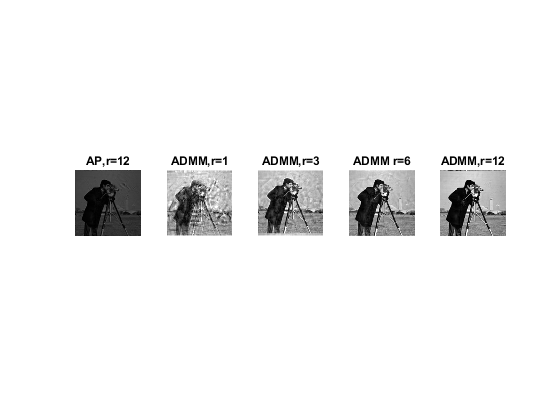
\includegraphics[width=12cm]{figures/ex1_u.png}%[]里可以指定影像大小
    \caption{Images reconstructed}    % 图名
    \label{1}  % 用于内部引用的图名
\end{figure}
\begin{figure}[H]   % 必须要有[h]否则插入的图片都在文字前面
    \centering  % 图像居中
    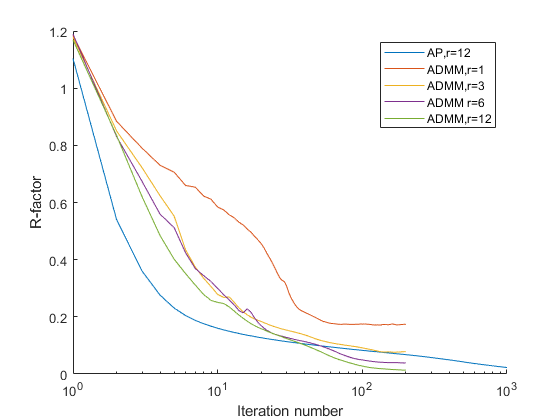
\includegraphics[width=12cm]{figures/ex1_R.png}%[]里可以指定影像大小
    \caption{R-factor, 200 iterations for ADMM and 1000 for AP}    % 图名
    \label{1}  % 用于内部引用的图名
\end{figure}

\subsection{Experiment for model\eqref{target}}
We set $\kappa$ as guassian kernel with variance $(\sigma_1,\sigma_2)=(7,0),(5,5)$. Here we use $gridFlag=1$, and we can see the periodical artifects. It seems that 3 modes are enough in this case.

\begin{figure}[H]   % 必须要有[h]否则插入的图片都在文字前面
    \centering  % 图像居中
    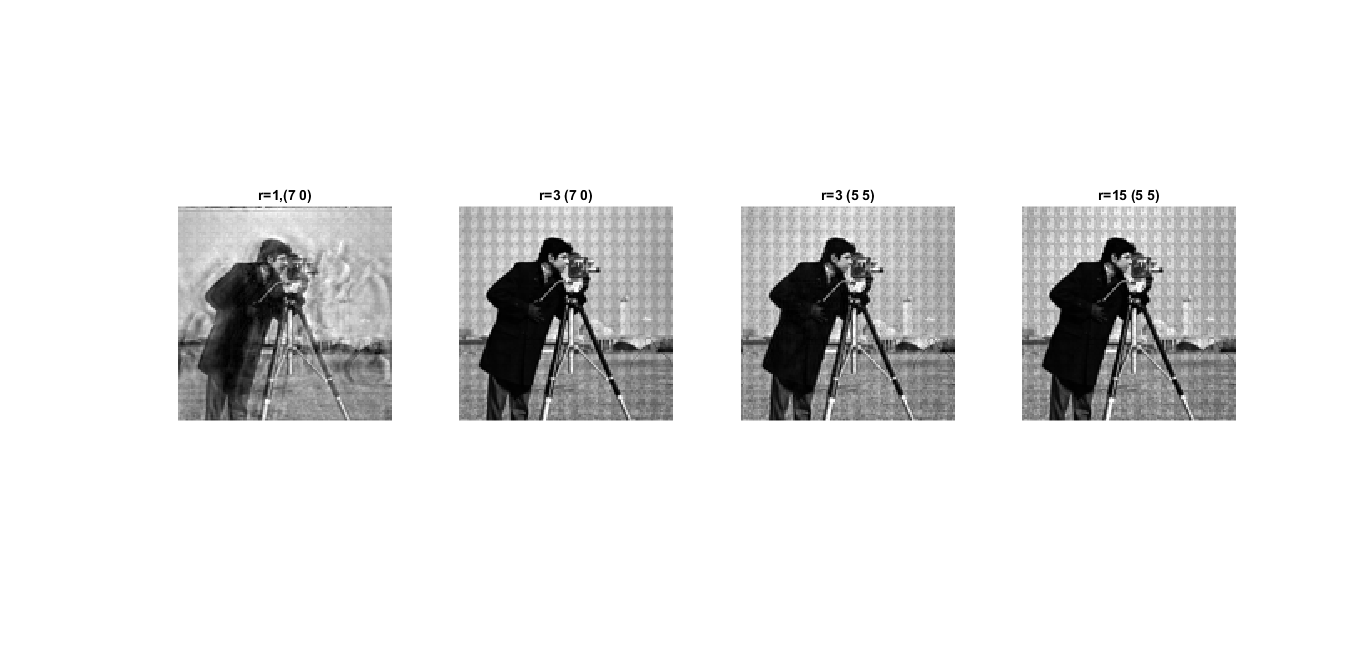
\includegraphics[width=12cm]{figures/ex2_u_2.png}%[]里可以指定影像大小
    \caption{Images reconstructed}    % 图名
    \label{1}  % 用于内部引用的图名
\end{figure}
\begin{figure}[H]   % 必须要有[h]否则插入的图片都在文字前面
    \centering  % 图像居中
    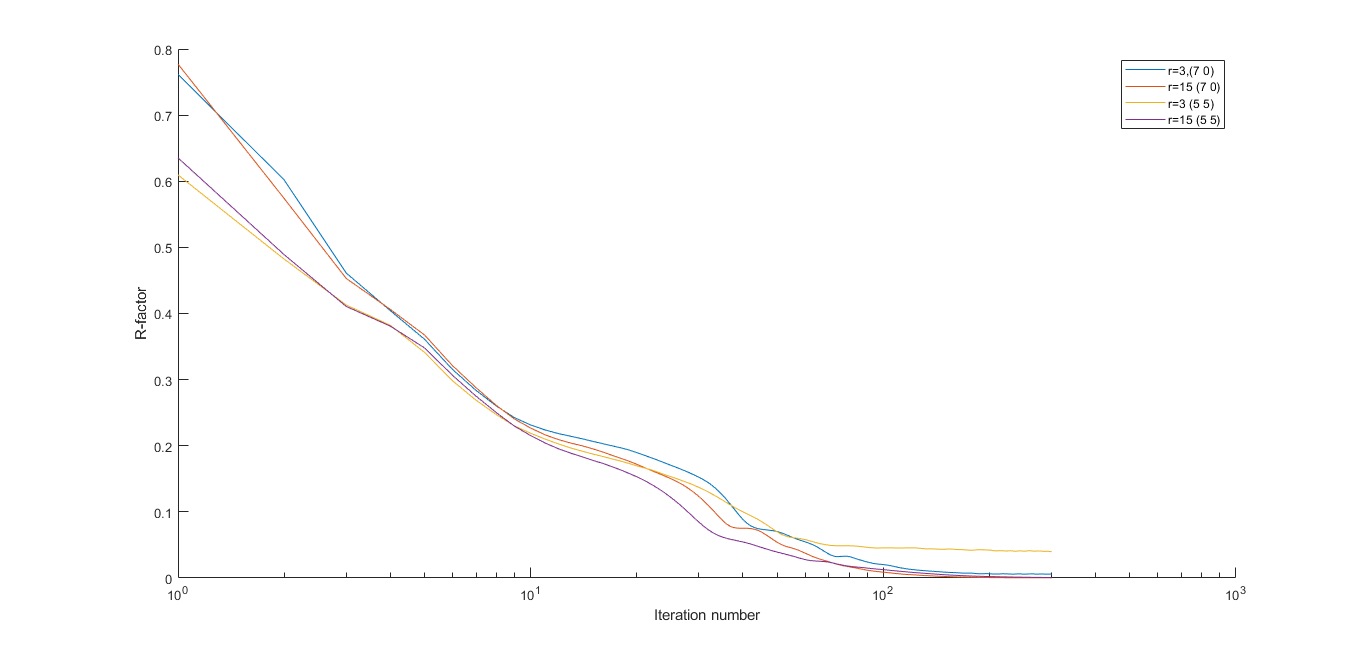
\includegraphics[width=12cm]{figures/ex2_R.png}%[]里可以指定影像大小
    \caption{R-factor, 300 iterations}    % 图名
    \label{1}  % 用于内部引用的图名
\end{figure}
And we generate standard modes from \eqref{section:reference}:
\begin{figure}[H]   % 必须要有[h]否则插入的图片都在文字前面
    \centering  % 图像居中
    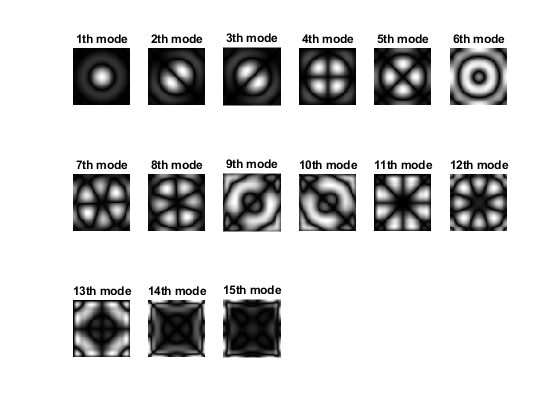
\includegraphics[width=8cm]{figures/ex_2_standard.png}%[]里可以指定影像大小
    \caption{standard modes}    % 图名
    \label{1}  % 用于内部引用的图名
\end{figure}

The modes reconstructed by our algorithm:
\begin{figure}[H]   % 必须要有[h]否则插入的图片都在文字前面
    \centering  % 图像居中
    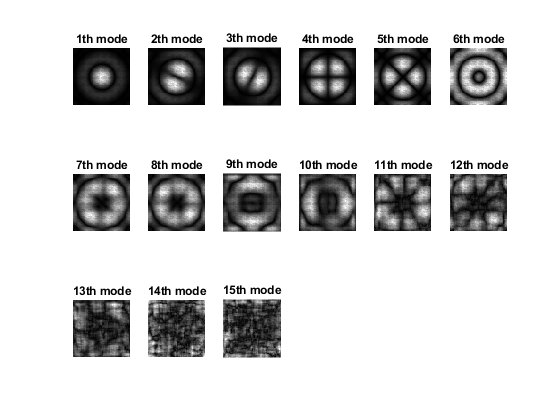
\includegraphics[width=12cm]{figures/ex_2_re.png}%[]里可以指定影像大小
    \caption{reconstructed modes}    % 图名
    \label{1}  % 用于内部引用的图名
\end{figure}
\begin{figure}[H]   % 必须要有[h]否则插入的图片都在文字前面
    \centering  % 图像居中
    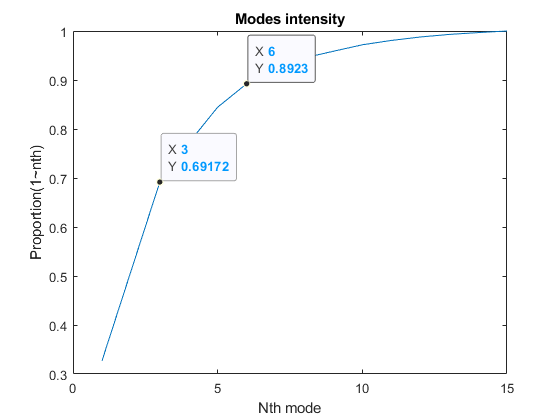
\includegraphics[width=8cm]{figures/modes_intensity_re.png}%[]里可以指定影像大小
    \caption{Mode intensities}    % 图名
    \label{1}  % 用于内部引用的图名
\end{figure}



%modes


%fig for blur effect



\section{Discussion and task}

\begin{enumerate}
\item Add orthogonal constraint in ADMM

\item Finish the proof in \ref{section:reference} QU. 


\end{enumerate}

 

\section{Appendix}
\subsection{Subproblems in ADMM}
\subsubsection{$\omega$}
Essentially in this subproblem, each state $\omega_i=w(:,:,i)$ is independent. Then we can optimize each $w_i$ seperately.
 $$
 \omega_i^{k+1}=\arg \min _{\omega \in \mathcal{X}_{1}} \frac{1}{2} \sum_{j}\left\|\mathcal{F}^{-1} \hat{z}(:,:,j,i)^{k}-\omega(:,:,i) \circ \mathcal{S}_{j} u^{k}\right\|^{2}
 $$
 
 Essentially in this subsubproblem, each element in $w_i$ is independent.
 such that one just needs to solve the following 1D constraint quadratic problem:
$$
\omega_i^{k+1}(t)=\arg \min _{|x| \leq C_{\omega}} \rho_{t}^{k}(x).
$$
where
$\rho_{t}^{k}(x):=\frac{1}{2} \sum_{j}\left|\left(\mathcal{F}^{-1} \hat{z}(:,:,j,i)^{k}\right)(t)-x \times\left(\mathcal{S}_{j} u^{k}\right)(t)\right|^{2} \forall x \in \mathbb{C}$ 

The derivative of $\rho_{t}^{k}(x)$ is calculated 
\footnote{Notice that here $\rho$ is a real value funtion with complex variable, and we use wirtinger derivatives here. More properties and calculation rules are listed in this link: \url{https://blog.csdn.net/weixin_37872766/article/details/107673096}} as
$$
\begin{aligned}
&\nabla \rho_{t}^{k}(x) = \dfrac{ d\rho_{t}^{k}(x)}{dx^*} \\
&\begin{aligned}
=\sum_{j}\left(x \times\left|\left(\mathcal{S}_{j} u^{k}\right)(t)\right|^{2}-\left(\mathcal{S}_{j} u^{k}\right)^{*}(t)\left(\mathcal{F}^{-1} \hat{z}_{j,i}^{k}\right)(t)\right)
\end{aligned} \\
&\begin{aligned}
=x \times\left(\sum_{j}\left|\left(\mathcal{S}_{j} u^{k}\right)(t)\right|^{2}\right)-\sum_{j}\left(\left(\mathcal{S}_{j} u^{k}\right)^{*}(t)\left(\mathcal{F}^{-1} \hat{z}_{j,i}^{k}\right)(t)\right) \\
\end{aligned}
\end{aligned}
$$
The first order optimality condition is $\nabla \rho_{t}^{k}(x)=0 $. Then the close form solution of $w_i$ is given as
$$
\omega_i^{k+1}=\operatorname{Proj}\left(\frac{ \sum_{j}\left(\mathcal{S}_{j} u^{k}\right)^{*} \circ\left(\mathcal{F}^{-1} \hat{z}_{j,i}^{k}\right)}{ \sum_{j}\left|\mathcal{S}_{j} u^{k}\right|^{2}} ; C_{\omega}\right)
$$

 





\begin{thebibliography}{99}
\bibitem{chang}{Chang, Huibin, et al. "Partially coherent ptychography by gradient decomposition of the probe." Acta Crystallographica Section A: Foundations and Advances 74.3 (2018): 157-169.}
\bibitem{theory}{New theory of partial coherence in the space–frequency domain Part I: spectra and cross spectra of steady-state sources}
\bibitem{mix}{Reconstructing state mixtures from diffraction measurements}
\bibitem{direct}{Multiplexed coded illumination for Fourier Ptychography with an LED array microscope.}
\bibitem{algorithm}{Probe retrieval in ptychographic coherent diffractive imaging}
\bibitem{quan}{Introduction to Quantum Mechanics, David J. Griffiths, 12.3}
\bibitem{all}{THE NUMERICS OF PHASE RETRIEVAL, ALBERT FANNJIANG AND THOMAS STROHMER}
\bibitem{admm}{Chang, Huibin, Pablo Enfedaque, and Stefano Marchesini. "Blind ptychographic phase retrieval via convergent alternating direction method of multipliers." SIAM Journal on Imaging Sciences 12.1 (2019): 153-185.}
\bibitem{psf}{An introduction to the theory of ptychographic phase retrieval methods}
\end{thebibliography}



\end{document}
